
	\subsubsection{Use-Case Instance - uciugStatisticAverageTypeofCrisis:ugAverageTypeofCrisis}
	
	The Administrator click the button to open the statistic so the system has to call the information for the average time of the different types and send it back to the Administrator so he can see it. 		  
	\begin{operationmodel}
	\addheading{usergoal Use-Case Instance}
	\adddoublerow{Instantiated Use Case}{ugAverageTypeofCrisis}
	\adddoublerow{Instance ID}{uciugStatisticAverageTypeofCrisis}
	
	\end{operationmodel} 

	
	Figure \ref{fig:lu.uni.lassy.excalibur.examples.icrash-RE-UC-uci-uciugStatisticAverageTypeofCrisis}
	The Administrator click the button to open the statistic so the system has to call the information for the average time of the different types and send it back to the Administrator so he can see it. 
	
	\begin{figure}[htbp]
	\begin{center}
	
	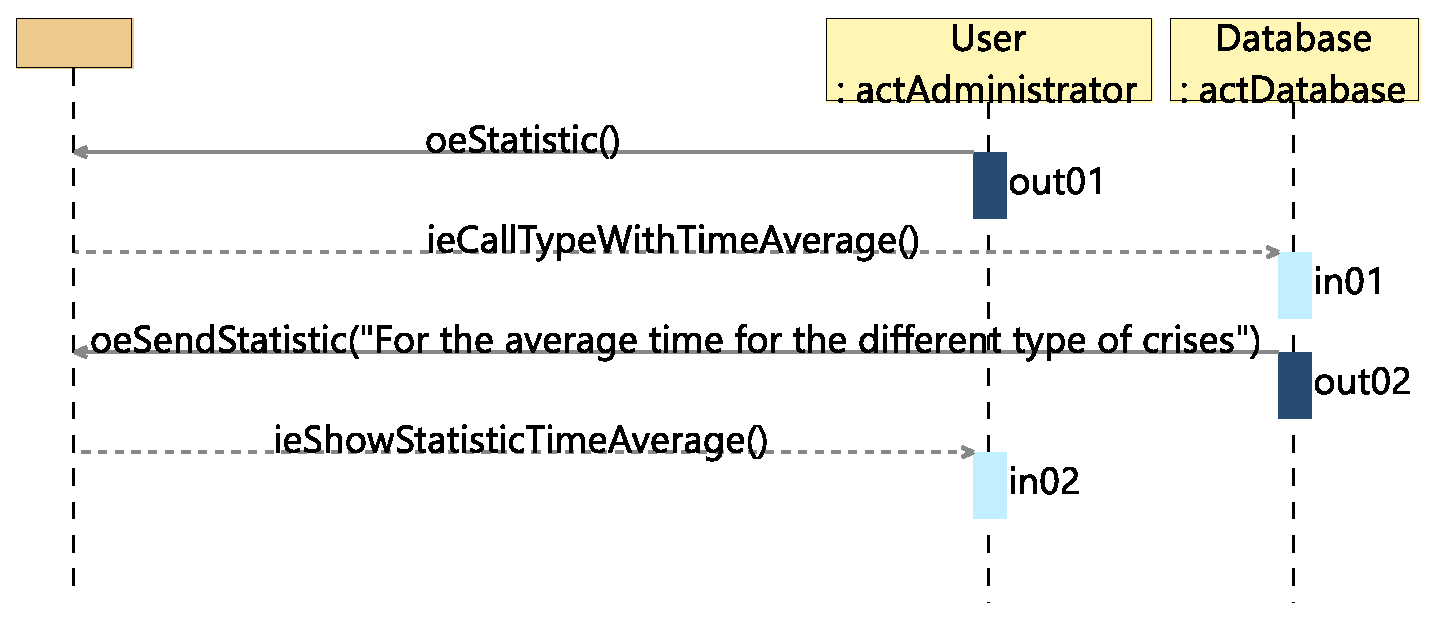
\includegraphics[
	angle=0
	,width=1.0\textwidth
	]{./images-report-gen/usecase-model/usergoal/uci-uciugStatisticAverageTypeofCrisis.eps}
	\end{center}
	\caption[lu.uni.lassy.excalibur.examples.icrash Sequence Diagram: uci-uciugStatisticAverageTypeofCrisis]{The average time of the different types}
	\label{fig:lu.uni.lassy.excalibur.examples.icrash-RE-UC-uci-uciugStatisticAverageTypeofCrisis}
	\end{figure}
	\vspace{0.5cm}
